%
% Modified version of the sample_ndthesis.tex
% by Sameer Vijay
% Last Change: Wed Jul 27 2005 14:00 CEST
%
%%%%%%%%%%%%%%%%%%%%%%%%%%%%%%%%%%%%%%%%%%%%%%%%%%%%%%%%%%%%%%%%%%%%%%%%
%
% Sample Notre Dame Thesis/Dissertation
% Using Donald Peterson's ndthesis classfile
%
% Written by Jeff Squyres and Don Peterson
%
% Provided by the Information Technology Committee of
%   the Graduate Student Union
%   http://www.gsu.nd.edu/
%
% Nothing in this document is serious except the format.  :-)
%
%%%%%%%%%%%%%%%%%%%%%%%%%%%%%%%%%%%%%%%%%%%%%%%%%%%%%%%%%%%%%%%%%%%%%%%%
% This is *not* a substitute for Donald's orginial documentation.  See
% /afs/nd.edu/usr/local/src/tex/texmf/doc/latex/ndthesis/ndthesis.dvi
% for documentation on the particular commands and whatnot.
%%%%%%%%%%%%%%%%%%%%%%%%%%%%%%%%%%%%%%%%%%%%%%%%%%%%%%%%%%%%%%%%%%%%%%%%
%
% You should *also* have a ND formatting guide to ensure that you have
% all the relevant parts, put the captions in the right place, etc.
% Just because you have this wonderful style classfile doesn't mean
% that it removes *all* the formatting onus from you.  :-)
%
% Normally, you should break all of this stuff up into separate files
% (at the very least, one chapter per file) and use the \input
% command.  This is all one file for brevity's (and clarity's) sake.
%
% Note that you should also have a good Makefile; one that invokes
% LaTeX as many times as necessary (up to 4) and bibtex if necessary.
% One should be included in this distribution.  You may want to modify
% the Makefile to make separate chapters, if necessary.
%
% If you have any suggestions, comments, questions, please send e-mail
% to: ndthesis@gsu.nd.edu
%
%%%%%%%%%%%%%%%%%%%%%%%%%%%%%%%%%%%%%%%%%%%%%%%%%%%%%%%%%%%%%%%%%%%%%%%%

\documentclass[textrefs,review]{nddiss2e}

% % uncomment the following line 
% if using chapter-wise bibliography
% \usepackage{chapterbib}
% \renewcommand{\bibname}{Cited Works}
% \renewcommand{\bibsection}{\section{\bibname}}

\begin{document}

\frontmatter

\title{GNUS AND YOU \\ {\small\scshape A BRIEF ON ALL AND EVERYTHING ABOUT GNUS IN OUR
SOCIETY} }
\author{Gerald G. Gnastich}
\work{Dissertation}
\degprior{B.S., M.S.}
\degaward{Doctor of Philosophy\\in\\Gnulogical Science}
\advisor{Gary Greenfield}
% \secondadvisor{Gordon Gray}
\department{Gnulogy}

\maketitle
%%%%%%%%%%%%%%%%%%%%%%%%%%%%%%%%%%%%%%%%%%%%%%%%%%%%%%%%%%%%%%%%%%%%%%%%
%
% Front stuff
%
%%%%%%%%%%%%%%%%%%%%%%%%%%%%%%%%%%%%%%%%%%%%%%%%%%%%%%%%%%%%%%%%%%%%%%%%

\copyrightholder{Garry Greene}
\copyrightyear{2005}
\makecopyright

\begin{abstract}
  Please note that the full \LaTeX\ source code (and an associated
  {\tt Makefile}) is available from the University of Notre Dame
  Graduate Student Union web site.  The Information Technology
  Committee page\footnote{{\tt http://www.gsu.nd.edu/}}
  has all the necessary files in download-able form.  This particular
  dissertation was developed under Unix, but should also be usable
  under Windows with the appropriate \LaTeX\ setup.  
  
  While the source code for this document provides an excellent
  example for how to use the \nddiss\ \LaTeX\ class to write a
  Notre Dame thesis, it is {\em not} a substitution for the
  documentation of the \nddiss\ \LaTeX\ class (also available on
  the ND GSU web site).

  In this thesis, I will tell all that I know about Gnus.  Gnus are
  wonderful little creatures that inhabit the center of the earth and
  give us wonderful and plentiful trees, dirt, and other
  earthly-things.
  
  In short, we should love and cherish the Gnus.  They can be very
  friendly, and are often mistaken for squirrels on the University of
  Notre Dame campus.  Feed them whenever possible.  If they get caught
  in trash cans, tip them over so that they can get out.

  This abstract is going to continue on, including a few formulas,
  just for the sake of spilling over on to two pages so that we can
  see the author's name in the top right corner:

  \begin{eqnarray*}
    a^2 + b^2 & = & c^2 \\
    E & = & mc^2 \\
    \frac{e}{m} & = & c^2 \\
    a^2 + b^2 & = & \frac{e}{m}
  \end{eqnarray*}

  These equations, by themselves mean nothing.  But to the common Gnu,
  they define a whole way of living.  While intricate mathematical
  implications certainly do not infiltrate the majority of humans'
  lives, every Gnu, from birth, is imbued with a sense of mathematical
  certainty and guidance.  All Gnus, great and small, feel at one with
  mathematics.  The cute furry bit is just a scam for their
  calculating minds.
\end{abstract}

\renewcommand{\dedicationname}{New Dedication Name}

\begin{dedication}
  To George, my favorite Gnu
\end{dedication}

\tableofcontents
\listoffigures
\listoftables

\begin{preface}
  I would like to preface this work with all the wonderful things that
  Gnus have brought to our society: trees, dirt, flowers, grass,
  lakes, and other earthly-things.  We should not forget them in our
  daily lives.

  Additionally, we should offer them food for all their hard work.  In
  fact, Gnus work so hard that they sleep for the colder half of
  the year.  As such, they tend to grow a little rotund.  Humans
  should not fault them for this, as it is necessary for their
  survival.  Indeed, many humans grow rotund on their on accord!
\end{preface}

\begin{acknowledge}
  I would like to acknowledge all the loving Gnus at Notre Dame.
  Particularly the one that comes to the window in the Hayes Healy
  building.  He (she?) has given me much inspiration, love, and dirt.
  I would also like to thank my advisor, Dr.\ Gary Greenfield, with
  whom this work would not have been possible.

  Finally, I would like to thank the U.S.\ Government, Department of
  Gnus, for their generous grant, number GNU3042920920.3, which
  allowed me to pursue my work.
\end{acknowledge}

\begin{symbols}
  \sym{\mathcal{F}}{sighting frequency of Gnus about campus}
  \sym{p}{student population}
  \sym{f}{type of food available}
  \sym{d}{day of week}
  \sym{c}{speed of light}
  \sym{m}{mass}
  \sym{e}{elementary charge}
  \sym{a,b}{miscellaneous constants}  
  \sym{E}{energy}  
\end{symbols}

\mainmatter

%
% Chapter 0 (features)
%
\setcounter{chapter}{-1}
\chapter{FEATURES OF FORMATTING IN THIS EXAMPLE FILE}

This \verb+chapter+ has been added to the original sample file to highlight the
various features with the formatting that conforms to the Graduate school
guidelines --- whether obtained due to the use of \nddiss\/ class file or just
plain good practice.
\begin{itemize}
\item An important thing you might notice is that the title of this chapter 
is not in all CAPS. This is a feature since using \verb+\MakeTextUpperCase{}+ 
is not helpful
when you have a math formula or something that just doesnt go CAPS (for eg.
elemental symbols).
\item If you're looking at a pdf document, the pdf bookmarks (left column) link
to all major textual sections including abstract, toc, lof, lot and
bibliography.
\item In the {\em dedication}, the title name has been modified. So, you know
how to and that it can be done.
\item The entries in the {\em List of figures} and {\em List of Tables} are
single-spaced themselves but are double-spaced from the other.
\item The table captions are not in all CAPS as well for the reason mentioned
above.
\item Appropriate space is left between the \verb+Table xx+ and its
corresponding caption (which is double-spaced itself) as in table \ref{tbl:bogus1}.
\item Tables look much better without the vertical lines (good practice).
\item There is double-spacing between the table entries but single-spacing
within the entry.
\item The chapter (see Chapter \ref{chap:golfing}) or section titles are
double-spaced as mentioned in the guidelines.
\item There is a \verb+subsubsection+ present (eg. section \ref{sec:data}) and
is properly formatted in the TOC.
\item Table \ref{tbl:defs} is an example of the use of \textsf{landscape}
environment in which a normal table is formatted in a {\em landscape} mode.
\item The \textsf{longtable} environment is used in Tables \ref{tbl:votes} and
\ref{tbl:rotated-rankings}, in normal and \verb+landscape+ mode, respectively. The
table captions are formatted properly in both cases.
\item In the table \ref{tbl:votes}, the \verb+footnote+ in the table header 
does not appear at all. This is not an error of the \nddiss\/ class but of the
\textsf{longtable} package.
\item An example of citing a website is shown in the bibliography (see
\citep{gairley2000}) which is formatted using the 
\verb+nddiss2e.bst+
citation style file.
\item A bit of information on the \nddiss\/ class file and the typesetting program
used is included in a box on the last page of the thesis.
\end{itemize}

%
% Chapter 1
%

%
% Modified by Sameer Vijay
% Last Change: Tue Jul 26 2005 13:00 CEST
%
%%%%%%%%%%%%%%%%%%%%%%%%%%%%%%%%%%%%%%%%%%%%%%%%%%%%%%%%%%%%%%%%%%%%%%%%
%
% Sample Notre Dame Thesis/Dissertation
% Using Donald Peterson's ndthesis classfile
%
% Written by Jeff Squyres and Don Peterson
%
% Provided by the Information Technology Committee of
%   the Graduate Student Union
%   http://www.gsu.nd.edu/
%
% Nothing in this document is serious except the format.  :-)
%
% If you have any suggestions, comments, questions, please send e-mail
% to: ndthesis@gsu.nd.edu
%
%%%%%%%%%%%%%%%%%%%%%%%%%%%%%%%%%%%%%%%%%%%%%%%%%%%%%%%%%%%%%%%%%%%%%%%%


%
% Chapter 1
%

\chapter{INTRODUCTION}

\section{Overview}

This is an overview of the introduction.  In here, I will use many
many buzzwords and other legalistic-types of terms, mostly begining on
the expounding of the holistic and synergistic energy that Gnus bring
to our organizations.

\subsection{Background}

In preparation for reading this dissertation, I would highly recommend
reading some of the other material available on
Gnus~\citep{gnus98:_gerry_ganst,greenfield96:_gettin_know_gnu}.  They
are very well written and will give you a fuller understanding of
Gnus.

Gnus are frequently mistakes for squirrels.  They are not squirrels.
They are Gnus.  Don't call them squirrels, either (unless you have
food in your hand); they tend to get a bit upset.\footnote{This is
  frequently mistaken for the chattering and scampering away.  Gnus
  are actually quite polite; they will leave if they have nothing nice
  to say, for fear of saying something offensive.}  If you have food
in your hand, they tend to ignore this insult and accept your food as
a peace offering.

\subsection{Foreground}

Table~\ref{tbl:bogus1} shows some feeding frequencies for where Gnus
like to eat around the Notre Dame campus.  Gnus have work weeks, just
like humans do, hence the much lower frequencies on weekends.  This
can lead us to conclude that Gnu weekend shifts are much smaller than
the normal work-week shifts.  In fact, we can attempt to parametrize the
sighting frequency, $\mathcal{F}$, by the student population, type of food, and
day of the week as:
\begin{equation}
  \mathcal{F} = \mathcal{F}(p,f,d).
\end{equation}
Table~\ref{tbl:bogus2} shows what they
typically like to eat.

\begin{table}[tpb]
  \begin{center}
    \caption{WHERE Gnus LIKE TO EAT \label{tbl:bogus1}}
    \begin{tabularx}{0.85\textwidth}{lrrrrrrr} \toprule
      \multicolumn{1}{c}{Location} & Sun & Mon & Tue & Wed & Thu & Fri & Sat \\ \midrule
      Front of Dome & 1 & 5 & 6 & 5 & 4 & 5 & 1 \\
      Stonehenge & 2 & 9 & 10 & 12 & 9 & 14 & 2 \\
      The Rock & 1 & 3 & 4 & 3 & 4 & 3 & 0 \\
      The ACC & 3 & 4 & 5 & 5 & 5 & 4 & 1 \\
      Dining Halls & 5 & 14 & 12 & 13 & 14 & 12 & 3 \\
      Hesburgh Library & 2 & 3 & 5 & 2 & 3 & 4 & 2 \\ \bottomrule
    \end{tabularx}
  \end{center}
\end{table}

\begin{table}[tpb]
  \setlength{\capwidth}{0.7\textwidth}
  \begin{center}
    \caption{WHAT Gnus LIKE TO EAT ON THE NOTRE DAME CAMPUS, LISTED
      BY AVERAGE NUMBER OF SIGHTINGS PER WEEKDAY
    \label{tbl:bogus2}
}
    \begin{tabular}{lrrrrrrr} \toprule
      \multicolumn{1}{c}{Food} & Sun & Mon & Tue & Wed & Thu & Fri & Sat \\ \midrule
      Twinkies & 1 & 5 & 6 & 5 & 4 & 5 & 1 \\
      Ding Dongs & 2 & 9 & 10 & 12 & 9 & 14 & 2 \\
      Carrots & 1 & 3 & 4 & 3 & 4 & 3 & 0 \\
      Lettuce & 3 & 4 & 5 & 5 & 5 & 4 & 1 \\
      Twizlers & 5 & 14 & 12 & 13 & 14 & 12 & 3 \\
      Jawbreakers & 2 & 3 & 5 & 2 & 3 & 4 & 2 \\ \bottomrule
    \end{tabular}
  \end{center}
\end{table}

Figure~\ref{fig:bogus3} shows a nice graph of location distributions
by day of week.  I have no real reason for including it except to show
that figures work as well.  Did I mention that Gnus are really cool?

\begin{figure}[tpb]
  \begin{center}
    \centerline{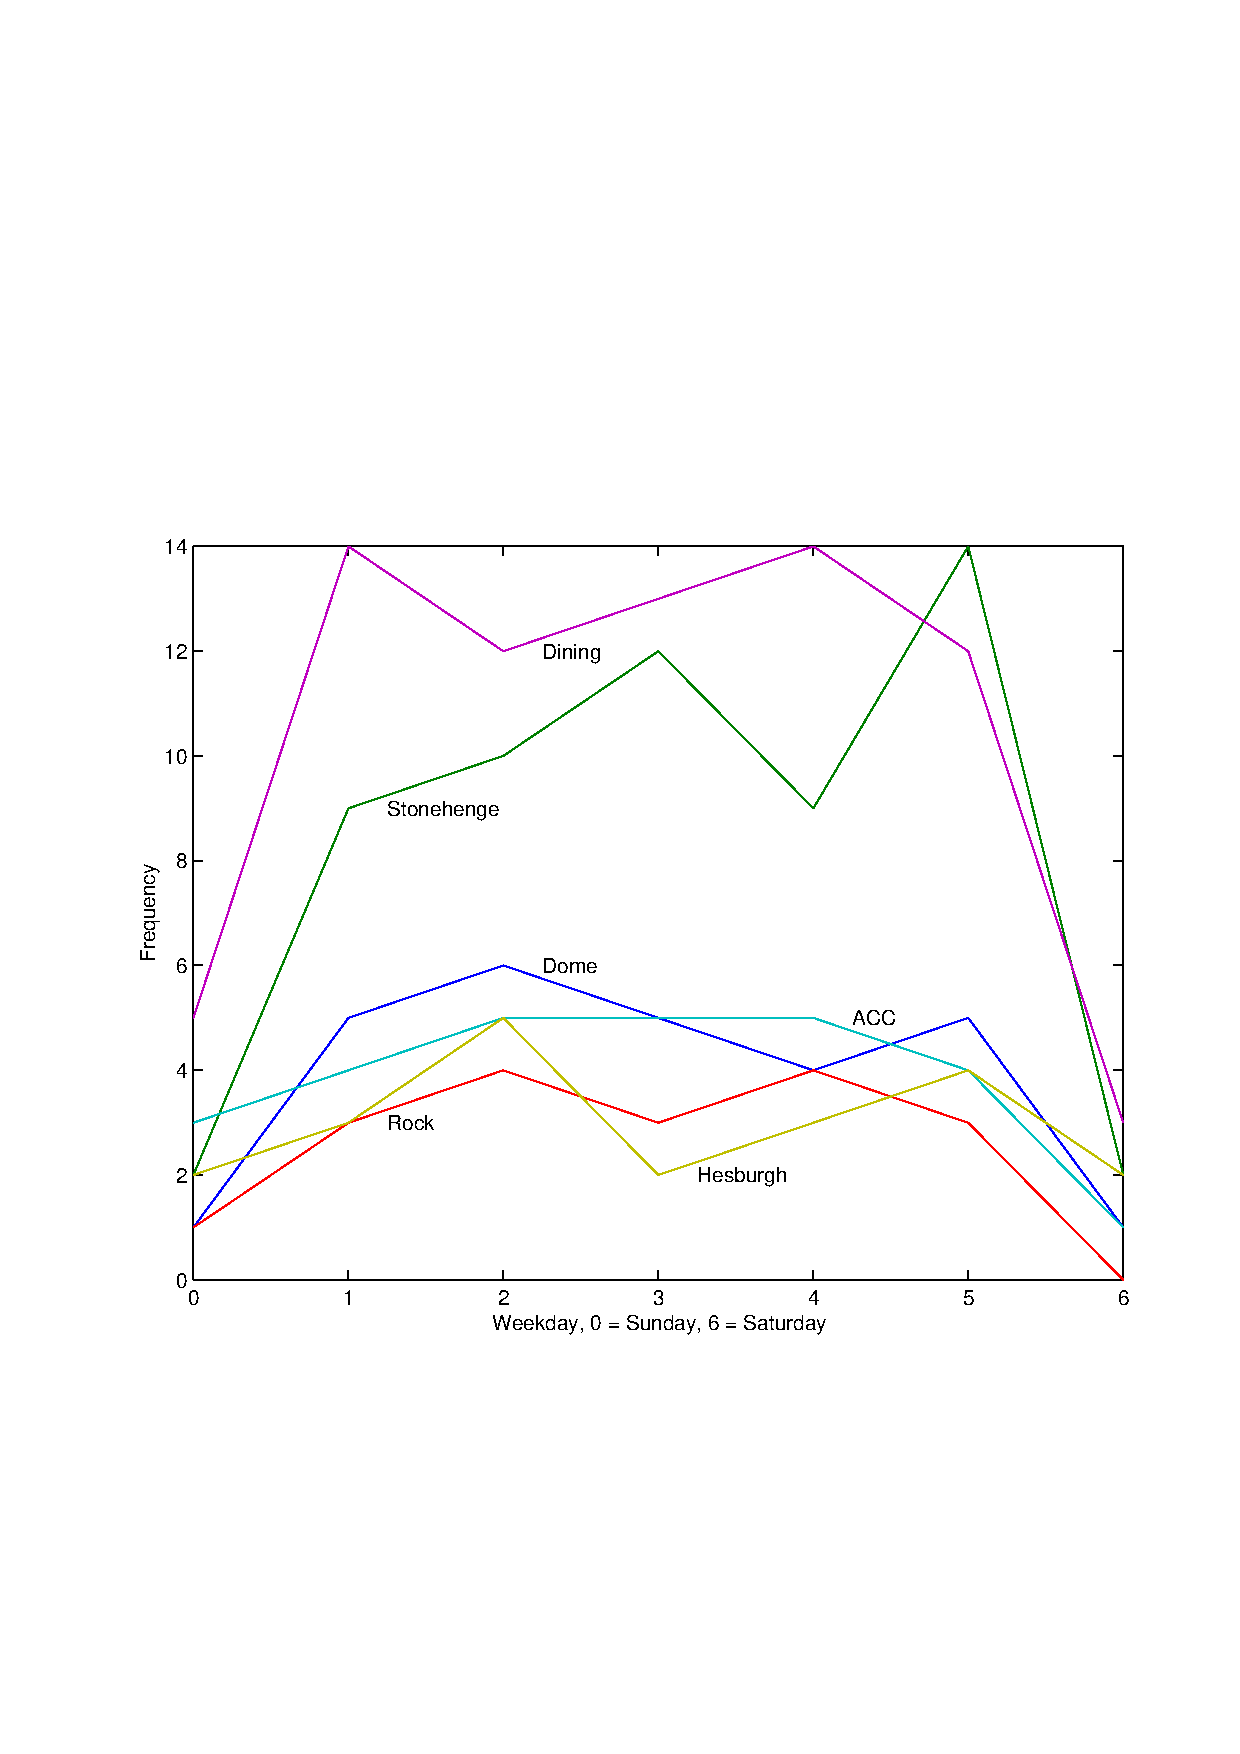
\includegraphics[scale=0.8]{sample_nd}}
    \caption{Location distributions by day of where, where the X axis
      is the weekday (0 through 6), and the Y axis is the sighting
      frequency}
    \label{fig:bogus3}
  \end{center}
\end{figure}

Gnus typically tend to come out when there are large gatherings of
humans with food.  Gnus work very hard at providing us with all the
things that we like (trees, dirt, air, etc.), and so we should freely
give them food.  They will come up and stand a respectful distance
away from you, waiting to see if they will be rewarded for their
efforts.  If you offer some food, they will take it and back off a
respectful distance in order to consume their food while leaving you
to your ``personal space.''  

\section{Groovin' Gnus}
\label{sec:groovin-gnus}

Gnus do tend to stay away from humans in their normal day-to-day
workings.  This is mainly because humans don't, for the most part,
understand what they are doing.  If a Gnu is working, and a human
approaches it, the Gnu will tend to drop whatever it is doing and run
away.  This is probably do to the tendency for humans to have ``group
meetings'' and ``productivity seminars.''  Most Gnus are deathly
afraid of such overmanagement, and run at the slightest hint of it,
for fear that it will cripple their real work.

It is interesting, however, that Gnus have chosen an Institution of
Higher Education for their BOO.\footnote{Base of Operations.}  It is
often said that:
\begin{quote}
  Academic politics are the dirtiest, meanest, ugliest, and generally
  the most low-down, in-your-face, and kick-em-while-they're-down than
  anywhere else (even Washington D.C.)  because the stakes are so low.
\end{quote}
It has been hypothesized that the Gnus are subtly trying to affect a
change for the better (i.e., eliminating the overmanagement problems)
by working the very system that they are trying to change, from
within.  That is, the graduates from Notre Dame can learn from the
examples of the Gnus here, and run screaming (or chattering) at the
slightest hint of overmanagement, and let the real work proceed
unhindered.

% % uncomment the following lines,
% if using chapter-wise bibliography
%
% \bibliographystyle{ndnatbib}
% \bibliography{example}



%
% Chapter 2
%

\chapter{فضاهای فشرده پایدار و فضاهای مرتب فشرده}
\thispagestyle{empty}
\section{فضاهای فشرده پایدار}
یک فضای توپولوژیک جزئاً مرتب (یا به طور خلاصه، فضای مرتب)، از دیدگاه آبرامسکی
\cite{abramsky2}،
مجموعه‌ای مانند $ X $ همراه 
با یک توپولوژی $ \mathcal{O} $ و یک ترتیب $ \leq $ است به طوری که گراف ترتیب در $X\times X  $ بسته باشد. بنابراین ...
\section{فضاهای مرتب فشرده}
در این  بخش به بیان ...


%
% Appendix
%

\appendix

%% Proposal appendix




%
% Back stuff
%

% % comment out the following three lines
% if using chapter-wise bibliography

 \backmatter
 \bibliographystyle{nddiss2e}
 \bibliography{example}

\end{document}

% End of ``example.tex''
